% fig:coverage-heatmap --- the tier-1 differential matrix as an example x backend
% heatmap. Cell status is the REAL per-(example,backend) status aggregated over
% schedules from nuc-nucleus/e2e-matrix.toml (P = all required cells pass; M =
% mixed, some schedule x backend cells skipped; s = all skipped). 26 examples
% appear in the tier-1 matrix (22-dma-pio-demo is embedded-only). Aggregate
% totals use the harness-verified macros. Grayscale-friendly (single-hue ramp).
\begin{figure}[tbp]
  \centering
  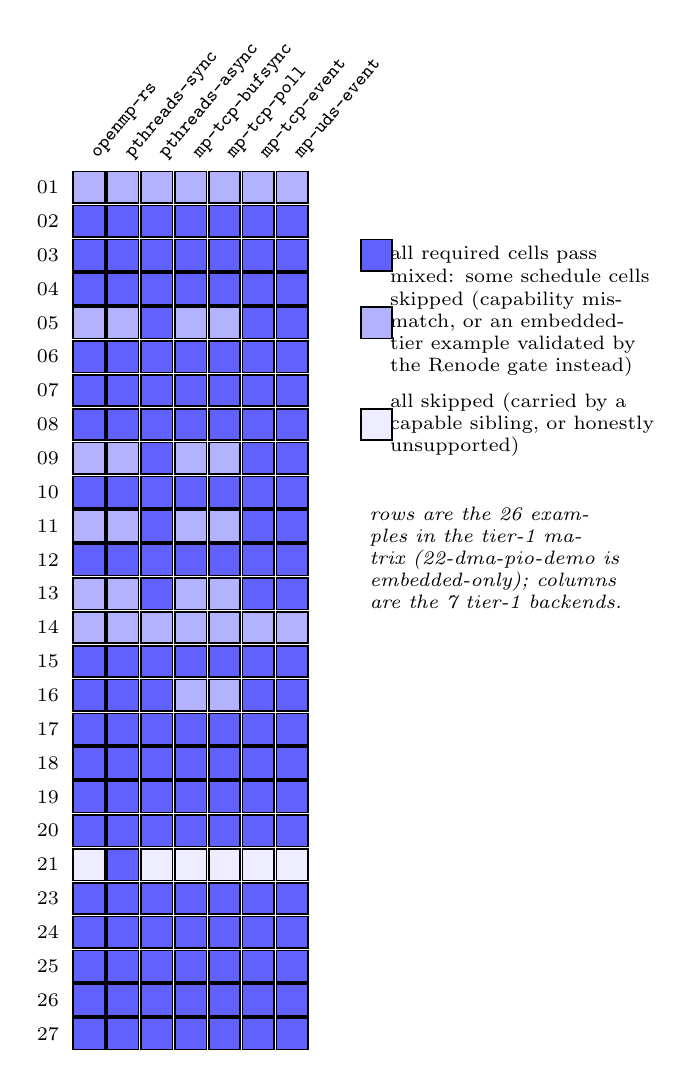
\begin{tikzpicture}[
      x=4.3mm, y=4.3mm,
      cell/.style={draw, semithick, minimum size=4.0mm, inner sep=0pt, anchor=center},
      P/.style={fill=blue!62}, M/.style={fill=blue!30}, s/.style={fill=blue!7},
    ]
    % backend column headers
    \foreach \be [count=\ci from 1] in {%
        openmp-rs, pthreads-sync, pthreads-async, mp-tcp-bufsync,
        mp-tcp-poll, mp-tcp-event, mp-uds-event}
      \node[rotate=50, anchor=west, font=\scriptsize\ttfamily] at (\ci, 0.7) {\be};
    % rows: example label + 7-cell status code (real data)
    \foreach \row/\lab [count=\ri from 0] in {%
        {M,M,M,M,M,M,M}/01, {P,P,P,P,P,P,P}/02, {P,P,P,P,P,P,P}/03,
        {P,P,P,P,P,P,P}/04, {M,M,P,M,M,P,P}/05, {P,P,P,P,P,P,P}/06,
        {P,P,P,P,P,P,P}/07, {P,P,P,P,P,P,P}/08, {M,M,P,M,M,P,P}/09,
        {P,P,P,P,P,P,P}/10, {M,M,P,M,M,P,P}/11, {P,P,P,P,P,P,P}/12,
        {M,M,P,M,M,P,P}/13, {M,M,M,M,M,M,M}/14, {P,P,P,P,P,P,P}/15,
        {P,P,P,M,M,P,P}/16, {P,P,P,P,P,P,P}/17, {P,P,P,P,P,P,P}/18,
        {P,P,P,P,P,P,P}/19, {P,P,P,P,P,P,P}/20, {s,P,s,s,s,s,s}/21,
        {P,P,P,P,P,P,P}/23, {P,P,P,P,P,P,P}/24, {P,P,P,P,P,P,P}/25,
        {P,P,P,P,P,P,P}/26, {P,P,P,P,P,P,P}/27} {
      \node[font=\scriptsize, anchor=east] at (0.4, -\ri) {\lab};
      \foreach \cell [count=\ci from 1] in \row
        \node[cell, \cell] at (\ci, -\ri) {};
    }
    % legend
    \node[cell, P, anchor=west] (lp) at (9.0, -2) {};
    \node[anchor=west, font=\scriptsize] at (9.6,-2) {all required cells pass};
    \node[cell, M, anchor=west] (lm) at (9.0, -4) {};
    \node[anchor=west, font=\scriptsize, align=left, text width=34mm] at (9.6,-4)
      {mixed: some schedule cells skipped (capability mismatch, or an
       embedded-tier example validated by the Renode gate instead)};
    \node[cell, s, anchor=west] (ls) at (9.0, -7) {};
    \node[anchor=west, font=\scriptsize, align=left, text width=34mm] at (9.6,-7)
      {all skipped (carried by a capable sibling, or honestly unsupported)};
    \node[anchor=west, font=\scriptsize\itshape, align=left, text width=34mm]
      at (9.0,-11) {rows are the 26 examples in the tier-1 matrix
      (22-dma-pio-demo is embedded-only); columns are the 7 tier-1 backends.};
  \end{tikzpicture}
  \caption[Tier-1 coverage heatmap]{The tier-1 differential matrix as an
    example-by-backend heatmap (rows are the 26 examples in the tier-1 matrix ---
    \texttt{22-dma-pio-demo} is embedded-only, hence the gap; columns are the
    seven tier-1 backends, of which \texttt{mp-uds-event} uses Unix-domain
    sockets). Each cell aggregates, over an example's schedules, its status on one
    backend: a dark cell (P) means every required schedule passes there, a mid
    cell (M) means some schedule is skipped, and a light cell (s) means all are
    skipped. Of \nmatrixtotal{} declared cells across the seven
    tier-1 backends, \nmatrixpass{} pass (emit, build, run, and reproduce the
    reference byte-for-byte), \nmatrixskip{} are skipped for a recorded reason ---
    the largest group embedded-tier fixtures validated by the simulator gate, the
    rest genuine capability mismatches carried by a capable sibling backend or a
    few honestly-unsupported language shapes --- and none fail. The broad band of
    dark cells is the cross-product of decompositions, IO disciplines, and
    runtimes exercised together on every build.}
  \label{fig:coverage-heatmap}
\end{figure}
